\documentclass{article}
\usepackage{graphicx}
\usepackage{float}
\usepackage{amsmath}

\title{Labwork 5: Gaussian Blur Convolution}
\author{Vu Ha Vy -- 2540112 \\}
\date{\today}

\begin{document}

\maketitle

\section{Implementation}

\subsection{Without Shared Memory}

In this implementation, each thread computes one pixel by reading directly from global memory. Every output pixel requires 147 global memory reads ($7 \times 7 \times 3$ color channels).

\subsection{With Shared Memory}

To improve performance, shared memory is used to store the $7 \times 7$ filter weights and the image block neighborhood. `cuda.syncthreads()` ensures threads complete loading data into shared memory before computing the convolution. \\

\noindent\textit{@cuda.jit} \\
\textit{def gaussian\_shared(src, dst, kernel):} \\
\textit{\hspace*{1.5em}tile = cuda.shared.array((7,7), dtype=np.float32)} \\
\textit{\hspace*{1.5em}tx = cuda.threadIdx.x} \\
\textit{\hspace*{1.5em}ty = cuda.threadIdx.y} \\
\smallskip
\textit{\hspace*{1.5em}if tx $<$ 7 and ty $<$ 7:} \\
\textit{\hspace*{3.0em}tile[ty, tx] = kernel[ty, tx]} \\
\smallskip
\textit{\hspace*{1.5em}cuda.syncthreads()} \\
\textit{\hspace*{1.5em}tidx = tx + cuda.blockIdx.x * cuda.blockDim.x} \\
\textit{\hspace*{1.5em}tidy = ty + cuda.blockIdx.y * cuda.blockDim.y} \\
\smallskip
\textit{\hspace*{1.5em}for c in range(3):} \\
\textit{\hspace*{3.0em}sum = 0.0} \\
\textit{\hspace*{3.0em}for ky in range(-3, 4):} \\
\textit{\hspace*{4.5em}for kx in range(-3, 4):} \\
\textit{\hspace*{6.0em}nx = min(max(tidx + kx, 0), src.shape[1] - 1)} \\
\textit{\hspace*{6.0em}ny = min(max(tidy + ky, 0), src.shape[0] - 1)} \\
\textit{\hspace*{6.0em}sum += (src[ny, nx, c]* tile[ky + 3, kx + 3])} \\
\textit{\hspace*{3.0em}dst[tidy, tidx, c] = np.uint8(sum / 1003.0)}


\section{Results}

\subsection{Qualitative Results}

\begin{figure}[H]
\centering
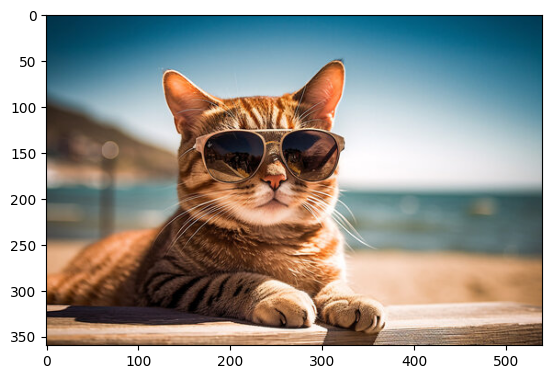
\includegraphics[width=0.45\textwidth]{images/input.png}
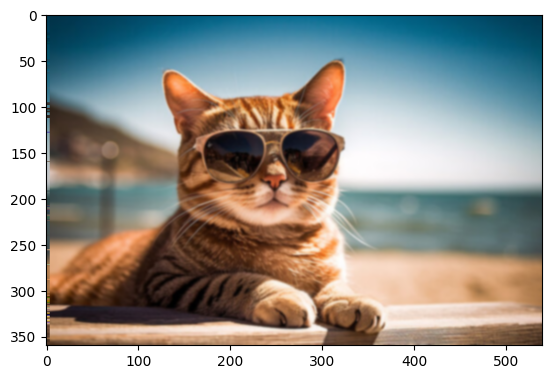
\includegraphics[width=0.45\textwidth]{images/blur.png}
\caption{Original image (left) and Gaussian blur output (right).}
\end{figure}
It successfully applies a Gaussian blur to the input image, smoothing out details.

\subsection{Quantitative Results}

We evaluated different 2D block sizes using both global memory (without shared memory) and shared memory implementations, obtaining the execution times shown below.

\begin{table}[H]
\centering
\begin{tabular}{|c|c|c|}
\hline
\textbf{Block Size} & \textbf{Without (s)} & \textbf{With (s)} \\ \hline
(8, 8)   & 0.0017311573028564453 & 0.00160980224609375 \\ \hline
(16, 16) & 0.0016818046569824219 & 0.00164031982421875 \\ \hline
(32, 8)  & 0.00165557861328125   & 0.001657247543334961 \\ \hline
(32, 16) & 0.0016489028930664062 & 0.0016486644744873047 \\ \hline
(32, 32) & 0.0019714832305908203 & 0.0019958019256591797 \\ \hline
\end{tabular}
\caption{Execution times across different block sizes.}
\end{table}

\begin{figure}[H]
\centering
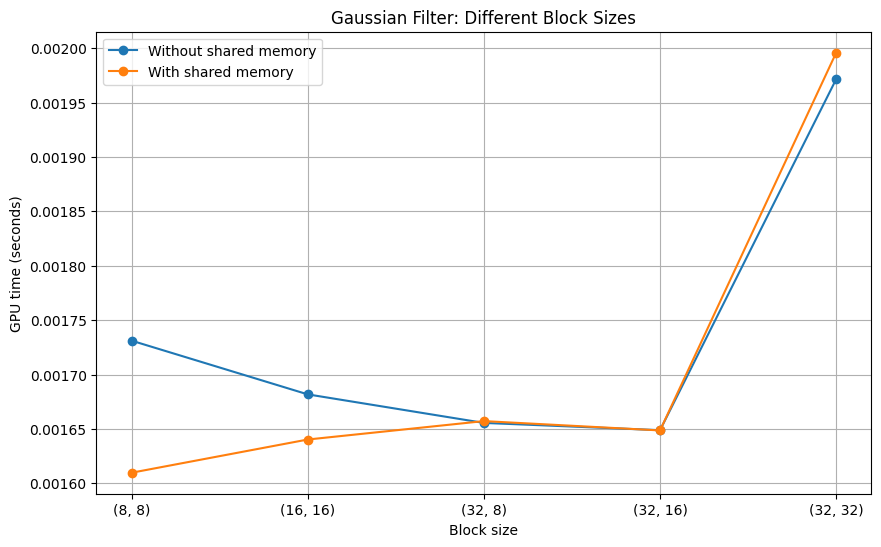
\includegraphics[width=0.7\textwidth]{images/compare.png}
\caption{Speedup comparison across different block sizes.}
\end{figure}

The fastest execution time of $0.00160980\,\text{s}$ was achieved using shared memory with a block size of $(8, 8)$. Shared memory provides a better performance for smaller block configurations such as $(8, 8)$ and $(16, 16)$. \\

Across configurations from $(16, 16)$ to $(32, 16)$, the running times remain quite similar with minimal difference between both versions. However, for $(32, 32)$ block size there is a large increase in execution time compared to $(32, 16)$ across both implementations due to maximum thread limits per block.

\end{document}